\chapter{L'algoritmo \emph{collapsed cone} e la sua implementazione in RayStation}
\setcounter{minitocdepth}{1}
\minitoc
\setcounter{minitocdepth}{2}
\textsf{In questo capitolo verrà descritto l'algoritmo di calcolo dosimetrico collapsed-cone-convolution e la sua implementazione all'interno del treatment planning system (TPS) \RS. Ci si soffermerà in particolare sugli aspetti riguardanti le approssimazioni intrinseche dell'algoritmo assieme alle approssimazioni adottate in fase di implementazione nel TPS. Ciò è propedeutico alla comprensione dei limiti e delle precisioni raggiungibili durante la modellizzazione di un fascio clinico per trattamenti radioterapici che verrà discusso nei capitoli successivi.}

\section{Introduzione}
Sin dagli albori della radioterapia la \textit{dose assorbita} è quella quantità che viene utilizzata al pari della dose farmacologica per ottenere un determinato effetto terapeutico. Più precisamente la definizione formale è fornita nel report ICRU n.85 \cite{ICRU85} come rapporto tra l'energia media $\de \bar{\varepsilon}$ impartita da radiazioni ionizzanti ad una massa $\de m$:
\begin{equation}
D = \frac{\de \bar{\varepsilon}}{\de m} \qquad\qquad \text{Unità: J\,kg}^{-1} \equiv \text{Gray [Gy]}
\end{equation} 
Esistono varie modalità di impartire una certa dose ad un paziente in radioterapia. Nell'ambito di questo lavoro si considererà solo la tecnica che fa impiego di fotoni generati da un acceleratore lineare (LINAC) denominata \virg{radioterapia a fasci esterni}.

Un LINAC è un'apparecchiatura in grado di accelerare elettroni fino ad energie dell'ordine dei 20 MeV che vanno a collidere su un target da cui si origina radiazione di frenamento (bremsstrahlung). Il fascio di fotoni così generato viene opportunamente filtrato e collimato per generare un fascio terapeutico. 
\begin{figure}
\centering
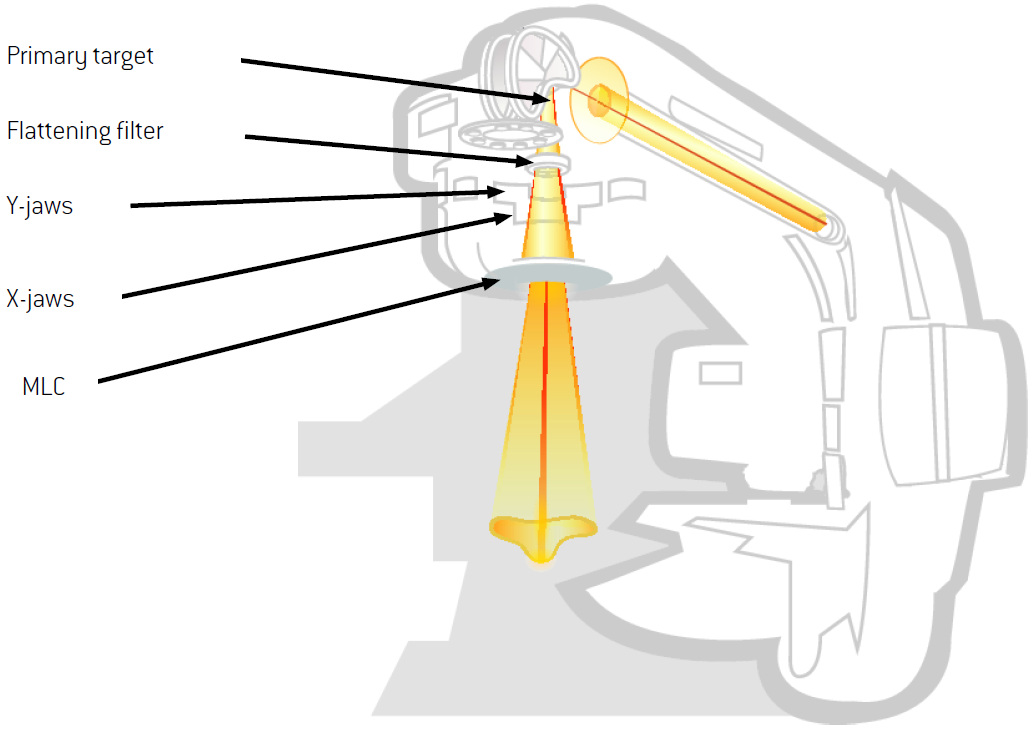
\includegraphics[width=.7\textwidth]{./cap1/linac.png}
\caption{Figura schematica di un acceleratore lineare per radioterapia a fasci esterni.}
\label{fig:linac}
\end{figure}
Tutto ciò si realizza nella testata del LINAC mediante l'uso di opportuni materiali schermanti che sono indicati nel disegno schematico riportato in Fig.\ref{fig:linac}.

Una volta che il fascio clinico investe il paziente, il meccanismo di deposizione della dose è un processo molto complesso dovuto alla grande quantità di processi che vengono innescati in cascata. \`{E} importante notare che una parte non trascurabile di processi avviene anche a livello della testata e questi vanno ad influenzare il fascio che effettivamente giunge al paziente. Ad esempio uno degli effetti più clinicamente rilevanti è la generazione di elettroni che \textquotedblleft contaminano\textquotedblright{} il fascio fotonico.

\begin{figure}
\centering
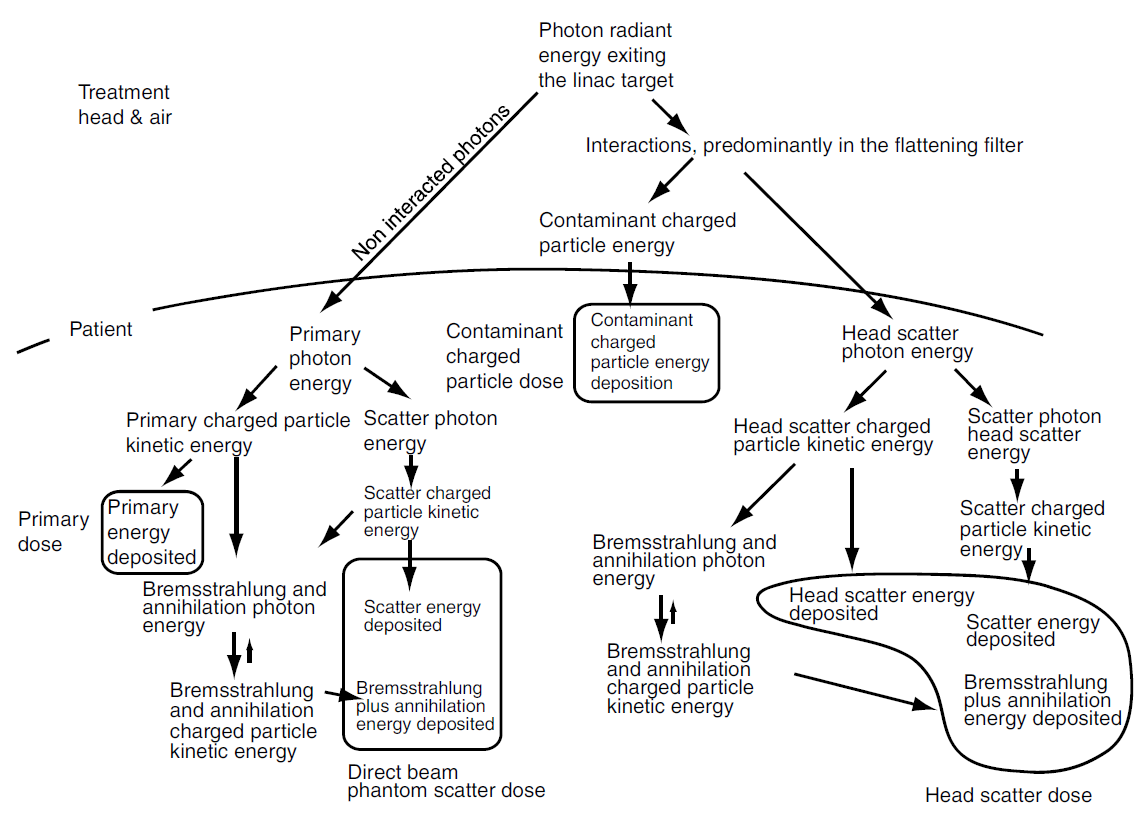
\includegraphics[width=.9\textwidth]{./cap1/processes.png}
\caption{Rappresentazione schematica delle principali interazioni che portano alla deposizione della dose nel paziente.}
\label{fig:processes}
\end{figure}
\vspace{.2cm}
La Fig.\ref{fig:processes} riassume schematicamente le principali interazioni che portano alla deposizione della dose nel paziente. \`{E} possibile identificare quattro principali meccanismi di rilascio della dose (cerchiati nella figura) che elenchiamo in ordine di importanza:
\begin{enumerate}
\item La dose primaria che rappresenta generalmente fino al 70\% della dose totale. Questa dose è generata dalla parte di fascio fotonico che non ha subito trasformazioni nella testata e che mette in moto particelle cariche le quali direttamente rilasciano la loro energia cinetica nella materia.
\item La dose di scatter dovuta al paziente (\textit{phantom scatter dose}) che può rappresentare fino al 30\% della dose totale. Questa componente è dovuta a tutti i processi di scatter che si innescano nel paziente a partire dal fascio primario come ad esempio fotoni di bremsstrahlung o fotoni scatterati per effetto Compton che portano ad una ionizzazione della materia con lo stesso meccanismo del fascio primario (messa in moto di elettroni).
\item La dose di scatter dovuta alla testata (\textit{head scatter dose}) che rappresenta generalmente il 5-10\% della dose totale. Questa parte della dose è dovuta al componente di fascio fotonico incidente sul paziente che ha subito interazioni nella testata (prevalentemente nel processo di filtraggio) e che presenta una distribuzione spaziale ed energetica differente dal fascio primario. Il meccanismo di rilascio dell'energia è esattamente analogo a quello del fascio primario.
\item La dose dovuta alle particelle di contaminazione del fascio fotonico che hanno un effetto rilevante (comparabile con il fascio primario) soltanto nei primi centimetri di tessuto. Questa zona è conosciuta come \textit{regione di build-up} della dose e vedremo in seguito il motivo.
\end{enumerate}


\section{Generalità sugli algoritmi di calcolo della dose al paziente per fasci di fotoni}
Un algoritmo di calcolo dosimetrico ha lo scopo di predire con un certo livello di accuratezza gli effetti presentati nella sezione precedente. In particolare il fine ultimo è predire la distribuzione di dose totale assorbita nel paziente che costituisce l'entità correlata all'effetto terapeutico sul tumore o al danno sul tessuto sano. La possibilità di prevedere questa quantità è propedeutica al processo noto come \textit{pianificazione del trattamento} in cui vengono adoperate delle opportune scelte riguardanti la collimazione e l'intensità del fascio volte a minimizzare il rapporto rischio/beneficio della terapia.

Esistono due grandi classi di algoritmi dosimetrici:
\begin{itemize}
\item Algoritmi \textit{correction-based}.
\item Algoritmi \textit{model-based}.
\end{itemize}
Gli algoritmi correction-based sono algoritmi empirici. Essi sono  basati su un gruppo di dati misurati in condizioni di riferimento (in un fantoccio ad acqua) e fanno uso di fattori o funzioni matematiche di tipo analitico o di tipo look-up-table per predire la distribuzione di dose assorbita in condizioni diverse da quelle di misura. 
Questi metodi furono i primi ad essere stati implementati in quanto non necessitano di grosse potenze di calcolo ma, d'altro canto, presentano dei limiti di accuratezza intrinseci per situazioni complesse (mezzi non omogenei, interfacce tra tessuti, campi di irradiazione molto irregolari o ad intensità modulata\ldots). Un'estensiva review di questi tipi di algoritmi è stata pubblicata da Fraass \textit{et al.}\cite{Fraass1995}.

\vspace{.2cm}
L'avvento della rivoluzione tecnologica e la crescita della potenza di calcolo disponibile tramite computer, ha permesso l'implementazione degli algoritmi model-based i quali simulano i processi di interazione radiazione-materia  a partire da principi primi tramite un modello fisico-matematico.\\
In questo caso il set di misure iniziali è unicamente utilizzato per ottimizzare i parametri del modello che poi viene applicato per predire la distribuzione di dose assorbita nei vari scenari clinici. Questi algoritmi hanno dimostrato una maggiore accuratezza rispetto ai correction-based ed al giorno d'oggi i più utilizzati sono quelli basati su tecniche di calcolo statistiche (Monte Carlo) o su metodi semi-analitici denominati algoritmi di convolution/superposition.

Il TPS RayStation in particolare implementa una tecnica di tipo convolution/superposition conosciuta come \textit{collapsed cone convolution} sviluppata a partire dalla metà dagli anni '80 indipendentemente da Mackie e Ahnesj{\"{o} \cite{Ahnesjo1989, Boyer1998, Mackie1985, Ahnesjo1987}.

\section{I principi di \textit{convolution} e \textit{superposition}}
continua qui con la presentazione di Gunter dell'Estro




















